% main.tex - IEEE ISAIA 2026 conference manuscript (6-page, two-column)
% "Evaluating Large Language Models for Automated Risk Register Generation
%  from Project Documentation: A Benchmark Study"
%
% Built on the official IEEE Conference Proceedings template
% (IEEE-conference-template-062824). Pure IEEEtran conference class: no
% journal-class overrides, no sidebar/footer macros, no \journal /
% \articletype / \backmatter. Submission via EasyChair; single-blind, so
% author identities are shown (not anonymized). Original, unpublished work.

\documentclass[10pt, conference, letterpaper]{IEEEtran}
\IEEEoverridecommandlockouts
\usepackage[T1]{fontenc}
% T1 is required, not cosmetic: the Limitations section cites "P\k{e}zik
% et al." (LLMLagBench); the ogonek \k{e} is a hard error under OT1.
\usepackage[utf8]{inputenc}
\usepackage{cite}
\usepackage{amsmath,amssymb,amsfonts}
\usepackage{graphicx}
\usepackage{booktabs}
\usepackage{array}
\usepackage{textcomp}
\usepackage{url}
\usepackage[hidelinks]{hyperref}

\begin{document}

\title{Evaluating Large Language Models for Automated Risk Register
Generation from Project Documentation: A Benchmark Study}

\author{%
\IEEEauthorblockN{Madhu Sudhan}
\IEEEauthorblockA{\textit{Dayananda Sagar College of Engineering}\\
Bengaluru, India \\
smadhu6364@gmail.com}
\and
\IEEEauthorblockN{Kruthik Jadhav}
\IEEEauthorblockA{\textit{School of Professional Studies} \\
\textit{New York University}\\
New York, NY, USA \\
kj2578@nyu.edu}
}

\maketitle

\begin{abstract}
No prior work benchmarks end-to-end risk-register generation against real,
published, human-authored ground truth across multiple large language
models; existing evaluations are almost entirely single-model and rely on
expert opinion rather than a genuine ground-truth artifact. We address this
gap with a benchmark of three models (one general-purpose proprietary model
and two architecturally distinct open-weight models), three prompting
strategies (zero-shot, few-shot, and structured reasoning), and 21
real-world projects that each have both public planning documentation and a
published human risk register (18 World Bank Project Appraisal Documents
and 3 UK government business cases), evaluated through a fully automated
pipeline: embedding-based semantic matching against ground truth as the
primary signal, and LLM-as-judge scoring as an explicitly supplementary,
non-human-substitute signal. Across 302 real, non-pilot runs, generated
registers recover 55.6 percent of ground-truth risks on average (mean
recall 0.556) while only 23.0 percent of generated risks correspond to a
real ground-truth risk (mean precision 0.230); among matched pairs, the
correct one of eight risk categories is assigned 45.0 percent of the time.
Model choice separates recall more cleanly than prompting strategy: the
proprietary model leads recall (0.612 to 0.693) with the fewest parse
failures, while the weaker-recall open-weight model instead has the highest
category accuracy and precision in most conditions, a conservative
generate-fewer-but-more-accurate pattern. Category-level analysis finds a
specific, non-uniform failure pattern rather than uniform weakness:
political and regulatory risk is the category models most often fail to
surface at all (191 of the 681 ground-truth risks missed corpus-wide, or
28.0 percent), while schedule risk is
generated as a near-default, safe category even where a project's real
register does not support it (238 hallucinated schedule risks, and the only
category for which no ground-truth risk is missed). We release the corpus manifest, extraction and prompting code, and
evaluation pipeline, including a disclosed account of the free-tier
provider constraints that shaped the timeline, so the benchmark is
reproducible.
\end{abstract}

\begin{IEEEkeywords}
large language models, project risk management, risk register generation,
reproducible benchmark, prompt engineering, hallucination detection,
category-level failure analysis, human-AI comparison
\end{IEEEkeywords}

\section{Introduction}

Risk registers are a high-value testbed for evaluating large language model
(LLM) generation against a real, structured, professionally authored
artifact. Unlike open-ended text, a risk register has a fixed, checkable
output contract (category, likelihood, impact, mitigation), and a
human-authored counterpart already exists for many appraised projects,
making semantic-matching evaluation against genuine ground truth possible.
Register quality is also not reducible to fluency: a well-written but
generic register, or one that hallucinates a plausible risk with no basis
in the project documentation, is a practical failure a project team could
act on badly.

LLMs are increasingly proposed for project-management tasks, yet the
literature concentrates on predictive analytics for time, cost, and quality
rather than generative capability \cite{aidriven2026usecases}. Work that
does study LLMs for project risk specifically has relied on expert-opinion
panels rather than comparison against real published artifacts, has been
almost entirely single-model (typically ChatGPT), and has not separated
\emph{generating} a full register from \emph{classifying} already-identified
risk items
\cite{asce2025exploring_chatgpt_risk,buildings2025risk_classification}. No
work has benchmarked multiple LLMs on end-to-end risk-register generation
from real project documents against published human-authored registers,
leaving both the accuracy and the systematic failure modes of this
capability unquantified.

We address this with three frozen research questions:
\begin{itemize}
\item \textbf{RQ1:} How complete and accurate are LLM-generated risk
  registers compared to human-authored ones?
\item \textbf{RQ2:} How do results vary across three models (one
  proprietary, two open-weight) and three prompting strategies (zero-shot,
  few-shot, structured reasoning)?
\item \textbf{RQ3:} Which risk categories do LLMs systematically miss or
  hallucinate?
\end{itemize}

This study makes four contributions: (i)~to our knowledge the first
benchmark of end-to-end risk-register \emph{generation} against real,
published, human-authored ground truth rather than expert opinion; (ii)~a
three-model comparison spanning a proprietary system and two
architecturally distinct open-weight models under three prompting
strategies, where prior work is almost uniformly single-model; (iii)~a
per-category failure-mode analysis (RQ3) that treats systematic omission
and hallucination as first-class findings rather than an aggregate accuracy
score; and (iv)~a released corpus manifest, extraction and prompting code,
and evaluation pipeline, with a disclosed account of the free-tier provider
constraints that shaped the experimental timeline (Section~\ref{sec:methods}).

\section{Related Work}
\label{sec:related}

\textit{AI in project management.} Systematic reviews consistently find
generative applications among the least-studied AI functions in the field,
with research concentrated on predictive analytics for schedule, cost, and
quality
\cite{aidriven2026usecases,aitools2025knowledge,salimimoghadam2025rise,leveraging2025ai_pm,mapping2025ai_landscape}.
Adoption is reported as limited by practitioners' unfamiliarity rather than
demonstrated capability gaps \cite{aitools2025knowledge}. The imbalance
motivating this study is thus a field-wide pattern, not an artifact of one
review's scope.

\textit{LLMs for project risk management.} The closest prior work evaluates
ChatGPT against expert judgment on construction-project risk
identification, finding strong performance on generic, checklist-style
risks but weaker performance on context-specific ones
\cite{asce2025exploring_chatgpt_risk}. Related studies report the same
generic-strong / specific-weak split under expert or focus-group
evaluation, though headline verdicts differ: one finds moderate performance
\cite{aladag2023assessing_chatgpt}, while a blind peer-review design finds
ChatGPT's scores exceed the human average even as reviewers still prefer
human answers for practicality \cite{ecam2024chatgpt_exceed_humans}.
Further work structures evaluation around ISO~31000
\cite{esrel2023iso31000_chatgpt} or builds a fine-tuned agent evaluated on
a few case studies \cite{wen2025riskgpt}. Across this line, three
limitations recur: single-model evaluation, no comparison against real
published ground-truth registers, and no public reproducible benchmark.

\textit{Classification vs.\ generation; prompting.} Classifying
already-identified risk items into categories is a related but materially
easier task \cite{buildings2025risk_classification,textmining2025scrm}: it
presupposes the risks are already identified, whereas end-to-end generation
requires a model to both identify and characterize risks from raw
documentation. RQ2's prompting comparison rests on two established results
treated here as background: in-context learning from a few demonstrations
without gradient updates \cite{brown2020fewshot}, and improved multi-step
inference from eliciting explicit reasoning before an answer
\cite{wei2022cot}. LLM-as-judge protocols are documented to be unstable and
subject to self-enhancement bias in expert domains
\cite{zheng2023judging_llm_judge,iui2025llmjudge_expert,nofreelabels2025,llmsasjudges2024survey},
which is why judge scoring here is strictly supplementary
(Section~\ref{sec:methods}). Table~\ref{tab:gap} summarizes how this study
differs from the closest prior work.

\begin{table}[t]
\caption{Gaps in Prior Work and How This Study Addresses Them}
\label{tab:gap}
\small
\begin{tabular}{@{}p{0.45\columnwidth}p{0.45\columnwidth}@{}}
\toprule
\textbf{Gap in Existing Work} & \textbf{This Study} \\
\midrule
Single-model, almost always ChatGPT & 3-model comparison incl.\ an open-weight model (RQ2) \\
Evaluated against expert opinion, not real ground truth & Semantic matching against published human registers (RQ1) \\
Construction-sector only & Cross-sector public corpus (World Bank + UK) \\
No public, reproducible benchmark & Corpus manifest, prompts, and code released \\
Known weak-category behavior never quantified per category & Per-category recall/precision failure-mode analysis (RQ3) \\
LLM-as-judge treated as an independent quality measure & LLM-as-judge reported strictly as a supplementary signal, never a human proxy (Section~\ref{sec:methods}) \\
\bottomrule
\end{tabular}
\end{table}

\section{Methodology}
\label{sec:methods}

\subsection{Corpus}
The corpus comprises 21 real-world projects that each have both public
planning documentation and a published, human-authored risk register: 18
World Bank Project Appraisal Documents (PADs) and 3 UK government business
cases (Five Case Model format). Each candidate had to clear four gates:
(1)~a structured, rated risk table is present; (2)~a substantive, itemized
narrative risk discussion beyond the table exists; (3)~the planning/risk
boundary is locatable and independently re-verifiable against the source
document; and (4)~at least 15 pages of planning content survive excision of
the risk content. Three candidates were read in full and excluded for
failing gate~(2) -- one also lacked any rated register at all, and one
HTML-only business case contained only two near-duplicate risks and could
not support per-category analysis; one UK project with 13 surviving
planning pages is retained as a disclosed exception to gate~(4). The 21
included projects span 18 sector labels (social protection, education,
energy and carbon capture, public health, public financial management,
water, transport, agriculture, digital identity, tourism, and others) -- a
deliberately cross-sector corpus rather than the single-domain (usually
construction) focus of prior LLM risk-evaluation work. The released
manifest records the planning-document URL and the ground-truth-register
URL as separate fields for every project.

\subsection{Leakage Control}
Because several source documents contain the human register in the same
file as the planning narrative, an author manually located each risk
section (e.g., the World Bank SORT table), excised it from the model input,
and recorded the exact page range removed; narrative passages restating the
register's risks were removed too. Every excision range was independently
re-verified against the source before ground truth was finalized, which
caught three under- and over-excision errors during construction. A
standing audit tool re-scans every document for heading and rated-table
patterns and checks each ground-truth risk's text for an 8-word
sliding-window phrase or distinctive code recurring verbatim in that
project's processed planning text. Its one flagged project was confirmed on
inspection to be a false positive (shared background text naming a
predecessor project, not risk content); we report this as the audit
working as intended, not as proof the corpus is leak-free by construction.

\subsection{Models and Experimental Grid}
Three models -- one general-purpose proprietary model and two
architecturally distinct open-weight models (Table~\ref{tab:models}) -- are
each evaluated under three prompting strategies across all 21 projects,
with 2 runs per cell at temperature 0--0.1: a $189$-cell $\times$ 2-run
grid. The open-weight pair is Meta's \texttt{Llama-3.3-70B-Instruct} and
OpenAI's \texttt{gpt-oss-120b}, an Apache-2.0 licensed Mixture-of-Experts
model; both are served through SambaNova Cloud's serverless API under the
exact identifiers in Table~\ref{tab:models}, with no local fine-tuning or
weight modification. Models receive planning documentation only; a
project's ground-truth register never enters its prompt or any few-shot
example (few-shot demonstrations are fully synthetic). The tier was originally meant to
include two proprietary models plus one open-weight model; it was changed
after all three original provider accounts proved unfunded on first use, a
real and disclosed change to the comparison's shape. All models run on
providers' free tiers (Google: 20 requests/day per model; SambaNova Cloud:
20 requests/min, 20 requests/day, and 200{,}000 tokens/day, each per
model), so the full grid is collected by repeated daily invocation over
roughly three weeks; the pipeline appends run metadata and a resumption
routine tops each cell up to its target count. On a transient rate-limit
the two open-weight rows fall back to OpenRouter (paid, same model
identifiers, US\$0.002--0.006/call); total real spend was about US\$0.18.
Free-tier responses from more than one provider were observed to spend part
of the output-token budget on hidden reasoning content, silently
truncating early runs until the budget was raised -- an output-budget
artifact easily mistaken for a model-quality difference, so disclosed
explicitly.

\begin{table}[t]
\caption{Model Lineup (Role, Dispatched Identifier, Provider)}
\label{tab:models}
\small
\begin{tabular}{@{}p{0.15\columnwidth}p{0.5\columnwidth}p{0.24\columnwidth}@{}}
\toprule
\textbf{Role} & \textbf{Dispatched Model} & \textbf{Provider} \\
\midrule
Proprietary & \texttt{gemini-flash-\allowbreak latest} (resolves to \texttt{gemini-\allowbreak 3.6-flash}) & Google, free tier \\
Open-weight \#1 & \texttt{gpt-oss-120b} & SambaNova, free tier \\
Open-weight \#2 & \texttt{Meta-Llama-\allowbreak 3.3-70B-\allowbreak Instruct} & SambaNova, free tier \\
\bottomrule
\end{tabular}
\end{table}

\subsection{Prompting Strategies and Output Schema}
The three strategies are grounded in the in-context-learning and
chain-of-thought literature (Section~\ref{sec:related}): \emph{zero-shot}
supplies only the task instruction and output schema; \emph{few-shot} adds
synthetic worked demonstrations \cite{brown2020fewshot}; \emph{structured}
additionally instructs the model to emit visible step-by-step reasoning
before a literal \texttt{FINAL JSON:} marker \cite{wei2022cot}. Each
generation is validated against a fixed JSON Schema
(\texttt{additionalProperties} disallowed at both levels). Every risk
object requires seven fields: a unique identifier; a free-text description;
exactly one of eight fixed categories (technical, financial, schedule,
stakeholder, political/regulatory, environmental, organizational,
external); likelihood and impact on a 1--5 integer scale; a mitigation; and
an evidence field, capped at 25 words, naming the specific
planning-document passage that motivated the risk. A generated risk with no
evidence traceable to the supplied planning text is the operational
definition of a hallucination for RQ3. An early version of the
structured-condition parser anchored a single greedy regular expression to
the end of the response and silently discarded all but the first JSON
value; caught after one cell showed an implausible 42-of-42
parse-failure rate, it was corrected against the immutable raw outputs
already on disk (never regenerating a call), recovering 39 of 88 grid-wide
parse failures. The remaining 49 were individually checked and are genuine
content issues (invalid categories, missing fields, or output truncation),
not parsing artifacts.

\subsection{Evaluation}
Evaluation uses an automated ground-truth signal and a supplementary
model-based signal. The original design also called for a third,
human-expert method (blinded practitioner ratings on a 45-register sample,
agreement via Fleiss' $\kappa$); that protocol was fully built and tested,
but recruiting the 3--5 raters did not prove feasible within the timeline,
so it is formally descoped (Section~\ref{sec:limitations}) rather than
replaced with an LLM judge standing in for the human baseline. The paper is
accordingly scoped as a fully automated evaluation, and both remaining
methods are re-runnable end-to-end from released code and already-public
data with no recruiting step.

\emph{Method A (primary): semantic matching.} Generated and ground-truth
risks within a project are embedded (\texttt{all-MiniLM-L6-v2}) and matched
greedily, highest-similarity-first, one-to-one, above a similarity
threshold validated against a hand-labeled set of risk-description pairs.
Matched pairs yield per-category recall (share of ground-truth risks
recovered) and precision (share of generated risks corresponding to a real
one); an unmatched generated risk with no traceable evidence field is a
candidate hallucination for RQ3.

\emph{Method C (supplementary only): LLM-as-judge.} The three dimensions
originally planned for human rating -- completeness, accuracy/plausibility,
and mitigation actionability, each 1--5 -- are also scored by an LLM judge
given the same inputs a human rater would have seen. With no human baseline
to validate against, Method C is reported strictly as a descriptive
secondary signal, never as an independent quality measure or a human proxy
(Section~\ref{sec:related}).

\subsection{Reproducibility}
Every generation call is logged to an append-only record capturing the
model version string, run date, sampling temperature and whether the
provider honored it, and the SHA-256 hash of the prompt file, alongside the
raw-output path; raw outputs are never overwritten, so a partially complete
grid can be resumed without duplicating or discarding a real call. The
corpus manifest, extraction and prompting code, output schema, and
evaluation pipeline are released so the full grid is independently
reproducible, subject to each provider's model-version rollover policy.

\section{Results}
\label{sec:results}

\texttt{results/raw\_outputs/} contains 392 real generations, with every
one of the 189 (project $\times$ model $\times$ prompt) grid cells covered
by at least 2 real runs. Results below are Method A unless noted, and
exclude a 5-project short-register subgroup (reported separately in
Section~\ref{sec:rq1-results}). A parse failure counts as recall $=0$ for
that run but is excluded from its precision and category accuracy (both
undefined with zero generated risks), so precision and category-accuracy
means are computed over fewer runs than recall in any cell with failures.

\subsection{RQ1: Completeness and Accuracy}
\label{sec:rq1-results}
Corpus-wide (302 runs), generated registers recover 55.6\% of ground-truth
risks on average (mean recall 0.556) while only 23.0\% of generated risks
correspond to a real ground-truth risk (mean precision 0.230); among
matched pairs the generated risk is filed under the correct one of eight
categories 45.0\% of the time (mean category accuracy 0.450). Across all
models and strategies, a generated register recovers roughly half of what a
human register contains, and roughly three-quarters of what it generates
matches nothing in the human-authored register (Fig.~\ref{fig:rq1}). This
is more cautious than the blind expert-review study whose reviewers scored
ChatGPT above the human baseline on the same task
\cite{ecam2024chatgpt_exceed_humans}; we attribute the difference to
evaluation design -- expert review scores reader-perceived plausibility,
whereas matching against a specific real register penalizes a risk that
corresponds to nothing in that exact document even if it reads sensibly.

The 5-project short-register subgroup (90 runs) sharpens the picture: mean
recall rises to 0.682 while mean precision collapses to 0.095. Models do
not shorten their output for a project whose real register is genuinely
short; they generate a similar volume regardless, so recall holds while
precision craters. This is evidence against a simple ``models
under-generate'' account and toward ``models do not calibrate output volume
to a project's real risk surface'' -- which matters for RQ3.

\begin{figure}[t]
\centering
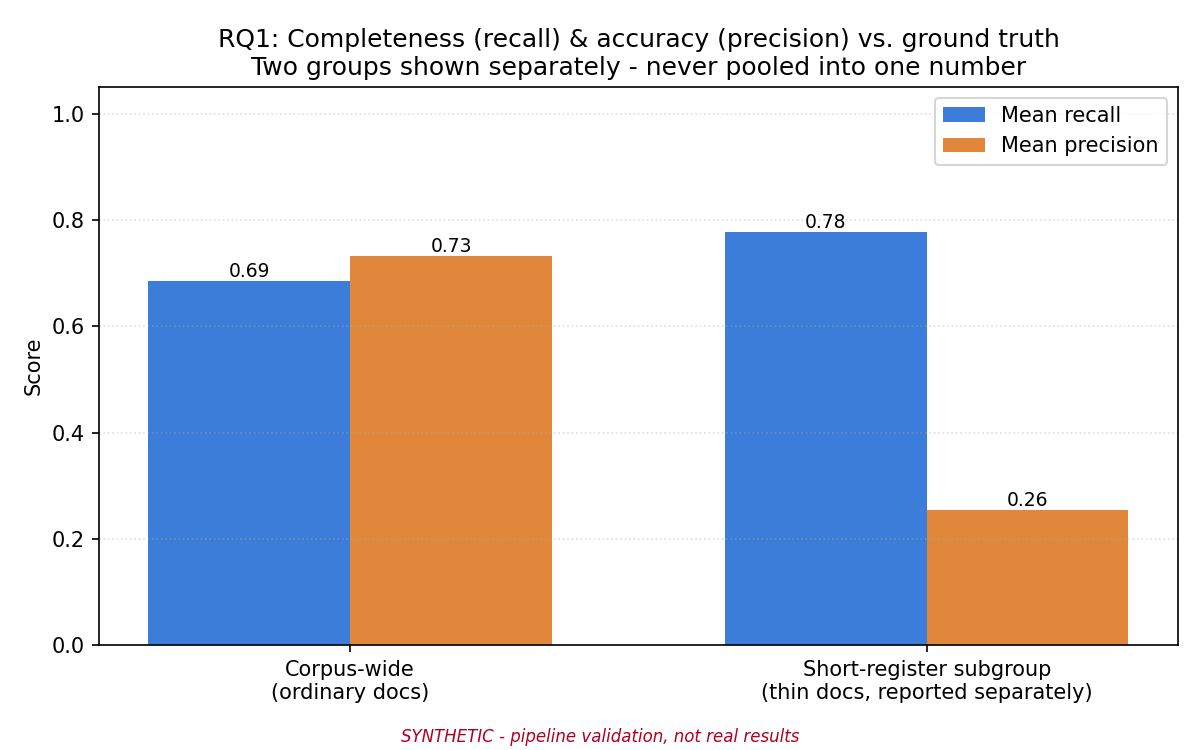
\includegraphics[width=\columnwidth]{../analysis/figures/fig_rq1_recall_precision.png}
\caption{Mean recall and precision, corpus-wide vs.\ the short-register subgroup, shown separately rather than pooled into one number (Section~\ref{sec:rq1-results}).}
\label{fig:rq1}
\end{figure}

\subsection{RQ2: Models and Prompting Strategies}
\label{sec:rq2-results}
Model choice separates recall more cleanly than prompting strategy
(Table~\ref{tab:rq2}). The proprietary model (Gemini) leads recall in all
three conditions (0.612--0.693) with the fewest parse failures (4.2\%
overall); Llama-3.3-70B trails in all three (0.408--0.494); gpt-oss-120b
sits between (0.521--0.614) but ties Llama on total parse failures (20 of
96 runs each, 20.8\%). Recall and category accuracy move in opposite
directions across models: Llama-3.3-70B has the lowest recall but the
highest category accuracy in every one of its conditions (0.456--0.630) and
the highest precision in two of three -- a conservative pattern (fewer
risks, but a larger share matched and correctly filed), the opposite
failure mode from a model that over-generates plausible but unmatched
risks. Structured prompting improves category accuracy for every model
(Gemini: 0.393 vs.\ 0.363--0.365; gpt-oss-120b: 0.503 vs.\ 0.450--0.474;
Llama-3.3-70B: 0.630 vs.\ 0.456--0.532) -- the clearest prompting effect in
the grid -- but its effect on recall is not consistent, so ``structured
reasoning helps'' holds here only for category accuracy.

\begin{table}[t]
\caption{Method A Results by Model and Prompting Strategy (Corpus-Wide, Excl.\ Short-Register Subgroup; 32 Runs/Cell)}
\label{tab:rq2}
\centering
\resizebox{\columnwidth}{!}{%
\begin{tabular}{@{}llrrrr@{}}
\toprule
\textbf{Model} & \textbf{Prompt} & \textbf{Fail} & \textbf{Rec.} & \textbf{Prec.} & \textbf{Cat.\ Acc.} \\
\midrule
Gemini (proprietary) & zero-shot & 2 & 0.675 & 0.229 & 0.365 \\
Gemini (proprietary) & few-shot & 1 & 0.693 & 0.245 & 0.363 \\
Gemini (proprietary) & structured & 1 & 0.612 & 0.229 & 0.393 \\
gpt-oss-120b (open-wt.\ \#1) & zero-shot & 5 & 0.614 & 0.196 & 0.450 \\
gpt-oss-120b (open-wt.\ \#1) & few-shot & 8 & 0.521 & 0.183 & 0.474 \\
gpt-oss-120b (open-wt.\ \#1) & structured & 7 & 0.539 & 0.202 & 0.503 \\
Llama-3.3-70B (open-wt.\ \#2) & zero-shot & 5 & 0.494 & 0.243 & 0.456 \\
Llama-3.3-70B (open-wt.\ \#2) & few-shot & 10 & 0.409 & 0.258 & 0.532 \\
Llama-3.3-70B (open-wt.\ \#2) & structured & 5 & 0.408 & 0.274 & 0.630 \\
\bottomrule
\end{tabular}}
\end{table}

\subsection{RQ3: Category-Level Failure Modes}
\label{sec:rq3-results}
Table~\ref{tab:rq3} gives missed and hallucinated counts by category.
Political/regulatory risk is the category models most systematically fail
to identify: 191 ground-truth political/regulatory risks have no matched
generated counterpart -- 28.0\% of the 681 ground-truth risks missed
corpus-wide, and more than any other category -- while its hallucination
count (163) is comparatively low, so models are not mislabeling other risks
as political/regulatory, they are simply not surfacing it as often as a
human author does. Schedule risk shows the opposite pattern in pure form:
it is the only category for which no ground-truth risk is missed, yet 238
generated schedule risks have no ground-truth match -- a near-default, safe
category models emit even when the project's real register does not support
it. Financial (497), technical (511), and
stakeholder (426) have the highest hallucination counts but, unlike
schedule, also have real missed counts (130, 69, 30), so their story is
over-generation alongside genuine omission. The ``other'' row (10 missed, 0
hallucinated) is a small set of ground-truth risks whose human category did
not map onto the fixed taxonomy; nothing is scored into it by design, so
its zero is mechanical. Read with the short-register finding
(Section~\ref{sec:rq1-results}), RQ3 is a story of poor calibration rather
than uniform weakness: models under-surface a category that needs close
reading of a project's specific governance context, while over-generating
categories that are safe generic completions of almost any planning
narrative.

\begin{table}[t]
\caption{Missed and Hallucinated Risks by Category (Corpus-Wide, Excl.\ Short-Register Subgroup)}
\label{tab:rq3}
\small
\begin{tabular}{@{}p{0.56\columnwidth}rr@{}}
\toprule
\textbf{Category} & \textbf{Missed} & \textbf{Hallucinated} \\
\midrule
Political/Regulatory & 191 & 163 \\
Financial & 130 & 497 \\
External & 110 & 205 \\
Organizational & 94 & 372 \\
Technical & 69 & 511 \\
Stakeholder & 30 & 426 \\
Environmental & 47 & 357 \\
Schedule & 0 & 238 \\
Other (non-taxonomy, ground truth only) & 10 & 0 \\
\bottomrule
\end{tabular}
\end{table}

\subsection{Method C: LLM-as-Judge Pilot}
A bounded feasibility pilot ($n=5$) ran the judge against real generated
registers for the first time; the same free-tier daily quota applies, and
the pilot deliberately drew only from \texttt{gpt-oss-120b} and
Llama-3.3-70B generations to sidestep self-preference bias (the configured
judge is the Gemini model also under test). Two of five calls (40\%)
returned a valid score (both \texttt{gpt-oss-120b}/zero-shot: completeness
5/5, accuracy 5/5, actionability 4--5/5); three (60\%) failed, two
truncated mid-JSON and one empty -- consistent with the same
hidden-reasoning-token truncation seen in the main grid, here against
\texttt{judge.py}'s smaller 512-token budget. With two successes from one
model-strategy cell the pilot supports no comparison claim; it is reported
only as evidence the pipeline produces a real score and that the judge
token budget must be enlarged before a full Method C run. The five raw
pilot outputs are released.

\section{Limitations}
\label{sec:limitations}

\textit{Pretraining contamination.} The corpus is public, so models may
have seen the documents -- including the held-out registers -- during
pretraining; excision controls the prompt, not prior training. The
Gemini-slot model's confirmed cutoff is March 2026 (only 4--5 months before
the run), Llama-3.3-70B's is December 2023, and gpt-oss-120b's is
unresolved across three non-agreeing sources (behavioral estimate September
2023, declared July 2024, self-report September 2021, per LLMLagBench,
P\k{e}zik et al.). A supplementary before/after-cutoff comparison, run
twice across the plausible gpt-oss-120b range and giving identical buckets,
finds pre-cutoff runs average \emph{lower} recall (0.435 vs.\ 0.585) and
higher precision (0.278 vs.\ 0.219) than post-cutoff -- the opposite
direction from a memorization story, in which a model that had memorized a
pre-cutoff register would show higher recall on exactly those documents. We
report this as evidence against the contamination hypothesis for this
corpus, not proof it did not occur; \texttt{publication\_date} is currently
populated for only 10 of 21 projects, and an automated backfill was
rejected because the World Bank's ``Expected Approval Date'' field records
a different concept.

\textit{Human ground truth is not a perfect oracle.} Method A measures
overlap with one published register; a low recall assumes that register is
itself complete, which is not guaranteed. Without the descoped
human-judgment signal, the study cannot separate a genuine generation gap
from a gap in the ground truth itself.

\textit{Threats to validity.} Method A's similarity threshold was validated
against hand-labeled pairs rather than real generations and should be
revisited if the corpus or embedding model changes. The Method C pilot's
60\% failure rate is a threat to that pilot's usefulness, traced to the
512-token judge budget rather than the judge model. Because the grid is
collected over multiple weeks of daily re-invocation, a provider-side model
rollover mid-collection would be visible in the per-call version logs but
would still threaten comparability across the boundary.

\textit{Method B descoping and ethics.} The blinded human-rating protocol,
sampling code, and blinded-packet pipeline are built, tested, and released,
but not run here; a future replication with recruiting capacity does not
have to rebuild them. All model inputs are already-public World Bank PADs
or UK government business cases -- no confidential or personally
identifying material -- and no human-subject data is collected. The
Gemini-slot free tier's terms permit provider use of unpaid-tier content
and human review; SambaNova's serverless policy is silent on training use.
Given already-public source material the practical sensitivity is limited,
but it is a real property of the setup.

\section{Future Work}
\label{sec:future-work}
Three directions follow from the results. First, the specific, non-uniform
failure pattern (under-surfacing political/regulatory risk; no
output-volume calibration) points toward retrieval-augmented or
taxonomy-grounded prompting as a targeted fix -- a fourth condition
evaluated with the same pipeline. Second, running the built-but-descoped
human-rating protocol would show where human judgments agree or disagree
with Method A at the level of individual registers, which Methods A and C
together cannot answer without a human baseline. Third, enlarging the judge
token budget and re-validating on a second small pilot would make a
full-corpus Method C run worthwhile, and re-running the released pipeline
against a larger or newer model roster -- once \texttt{publication\_date}
coverage is completed for all 21 projects -- would test whether this
recall/precision/category-accuracy pattern is specific to these models or
general to current LLMs.

\section{Conclusion}
We benchmarked three LLMs -- one proprietary, two open-weight -- under
three prompting strategies on end-to-end risk-register generation from real
planning documentation, evaluated against published human-authored
registers across 21 World Bank and UK projects. To our knowledge this is
the first benchmark of generation, rather than classification of
already-identified risks, against real ground-truth registers across
multiple models.

Generated registers recover about half of a human register's content (mean
recall 0.556) while roughly three-quarters of what they generate matches
nothing in it (mean precision 0.230); the short-register subgroup shows
this is a calibration failure, not a volume failure. Model choice separates
recall more than prompting strategy does, and the lowest-recall model is
the most precise and best-categorized -- a conservative failure mode
distinct from the higher-recall models' noisier output. Structured
prompting consistently improves category accuracy but not recall. The
category pattern is specific, not uniform: political/regulatory risk is
most often missed, schedule risk most often hallucinated -- evidence that
closing the gap needs targeted intervention, not simply larger models on
the same prompting comparison. The corpus manifest, code, and evaluation
pipeline are released, with a disclosed account of the free-tier
constraints and a corrected parser bug that would otherwise have fabricated
a full model collapse in one cell.

\section*{Data Availability}

The corpus manifest, extraction and prompting code, output schema,
matching/metrics/judging pipeline, and raw model outputs referenced in this
paper are released in the project repository at
\url{https://github.com/smadhu6364-beep/public-reproducible-benchmark}, per
the reproducibility commitments in Section~\ref{sec:methods}.

\section*{Acknowledgment}

This research received no external funding. The approximately US\$0.18 of
paid API fallback usage disclosed in Section~\ref{sec:methods} was covered
directly by the authors. The authors declare no conflict of interest.

\bibliographystyle{IEEEtran}
\bibliography{references}

\end{document}
